Carnatic and hindustani are two musical traditions in the indian subcontinent that are referred to as Indian Art Music (IAM), and whose common roots can be traced back to around 1000 BC\cite[p.15]{gulati}. They have many elements in common, but also notable differences. This chapter intends to provide a brief overview on carnatic music, in order to support a good understanding of the related work in chapter \ref{context}, and provide some basis to help the interpretation of the results of chapter \ref{conclusion}.\\

For that, it will cover first the aesthetical aspects that reflect the idiosyncrasy of its cultural context. This will help to understand the main features of the carnatic concert, the quintessential manifestation this music takes place in, described in the middle section. The last section of this chapter about carnatic music will describe the main elements of the proper musical discourse that are relevant in the context of the present thesis.


\section{Aesthetical Aspects}

Among the many artists present in the carnatic music corpus presented in \ref{about-ds}, Thodur Madabusi Krishna is present with six recorded concerts. Apart from playing carnatic music, he also captured his view of it in a book\cite{krishna}, in which he gives some insights that cana be helpful to understand the components and goals of carnatic music as a cultural phenomenon: ``Karnatik music is a most interesting form in its function within the social fabric and its own evolution. What makes it so is that its function is based on the musical aspects that constitute its existence. These are: raga, tala, composition and improvisation. The function of the musician is to express the various melodic and rhythmic aspects of the music with a complete understanding of its aesthetics and grammar. The musician is neither conveying a social message nor helping interpret a certain theatrical act or delivering a religious experience''\cite[p.30]{krishna}.\\

In fact, even when the music is featuring the human voice, he warns that, apart from the emotional and ideological dimensions that may take part in the artist's creative process, ``when presented in a Karnatik music concert, the focus is on the beauty of the language, its sounds, syllables and their interactions with the raga and tala'' because ``within the context of art music, there is no reason for the creation of music other than the music itself''\cite[p.33]{krishna}. And to clarify this focus even more, he finishes his thoughts on the matter with the following statement: ``Any discussion on the aesthetics of Karnatik music must be driven by this clear intent that the form has when presented as art music. Only such a discussion can lead us to a comprehensive understanding and give us the strength to question prevailing notions about Karnatik music''\cite[p.34]{krishna}.\\

The role of tradition also has a deep impact in the aesthetical aspects: ``Over the centuries, IAM has been orally transmitted across generations, following a hierarchical model of music training such as ghar\=an\=a (or school of music) [..]. Though the fundamental musical concepts used across ghar\=an\=as are the same, each ghar\=an\=a has its own ideology and characteristic style of music performance''\cite[p.16]{gulati}.\\

Such oral tradition does not only contribute to form different schools; it also conditions the evolution of the repertoire across the centuries: ``In Karnatik music, the word sampradaya means both conventions and traditions [...], all changes are considered to be within the spectrum of sampradaya. This gives all musicians the right to claim something as their sampradaya, while simultaneously abdicating the responsibility of comprehending these traditions, if at all they exist [...]. Many of the practices that we follow come under the category of convention, which are often the result of a single musician's actions. Once it is followed by her students and emulated by other musicians, it comes to be established as a sampradaya''\cite[p.13]{krishna}. So the concept of sampradaya poses a school-oriented context in which the different musical elements should take place and interact, and each individual artist has the responsibility of knowing it, as well as the liberty of altering it.\\

This, together with the virtuosism required by the interpretation itself, makes the practice of this repertoire a highly specialized task, so a small ensemble of solists became the natural way to play this music. Also as a consequence, the required attention to the details together with the polarization between interpreters and audience makes the concert an adequate way of delivering this music, and indeed the carnatic concert is the main format in which this music takes place.\\


Summarizing the considerations given so far, it can be said that the aesthetical discourse of carnatic music focuses on the purely musical forms, that are expressed by small ensembles of specialized soloists through the four constitutive aspects: r\=aga, t\=a\d{l}a, composition and improvisation (further elements would be by no means excluded from the performance, but wouldn't be  regarded as a part of the carnatic aesthetics). Also, that the evolution of the musical discourse is articulated through schools and, ultimately, by individual musicians, in a dynamic described via the concept of sampradaya.


\section{The Carnatic Concert}

As a consequence of the aspects above mentioned, it is easier to understand the fact that ``Carnatic music is a performance oriented music tradition, and mainly improvisatory in nature''\cite[p.16]{gulati}. This balance between individual and collective aspects has crystallised in a very specific set of formal conventions, that is known as the concert:\\

``In Carnatic music, a concert, also referred to as kach\=eri, is the natural unit of music performance. It is the unit typically considered for organization and digital distribution of Carnatic music content. A concert of Carnatic music typically comprises around 10 music pieces. Though Carnatic music is improvisatory in nature, the performances are based on compositions. Most of the compositions are to be sung, as a result of which, vocal music is dominant in Carnatic music. Even in instrumental music, artists aim to mimic vocal singing''\cite[p.16]{gulati}.\\

In addition to the formal aspects, the setup responds also to some common patterns:

``IAM is essentially heterophonic in nature, with a main melody being sung or played by the lead artist. Quintessentially, an instrument provides melodic accompaniment and follows the melody of the lead performer. A typical arrangement consists of a lead performer (in rare cases a duo), a rhythm accompaniment generally provided by  m\d{r}da\.{n}ga\.{m}, a constantly sounding drone in the background, and frequently, a melodic accompaniment using violin. The drone sound which is mainly produced by a t\=anpura is the only component that adds a harmonic element to the performance''\cite[p.16]{gulati}. Figure \ref{fig:instruments} pictures some of them.\\

\begin{figure}[h]
  \centering
  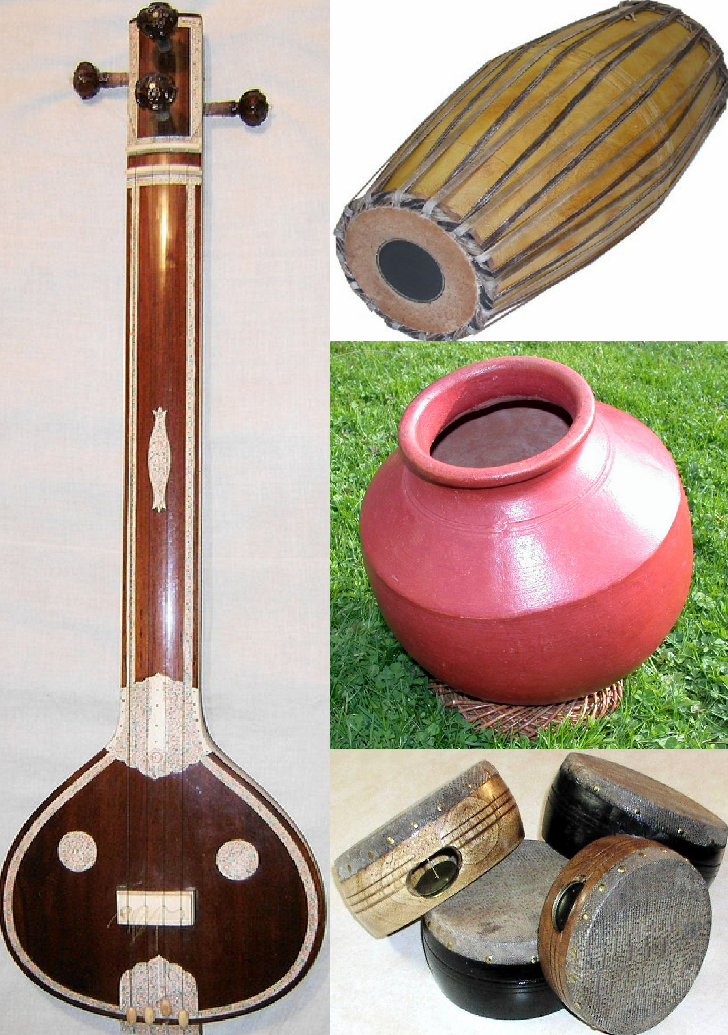
\includegraphics[scale=0.46]{instruments.png}
  \caption{The most popular non-melodic instruments that take part in a concert of carnatic music (Source: Wikipedia). Left: t\=anpura. Top: m\d{r}da\.{n}ga\.{m}. Middle: ghatam. Bottom: kanjira.}
  \label{fig:instruments}
\end{figure}



\section{Musical Elements}

So far, the main ideas and conditions that surround the actual musical elements have been exposed. From the four elements saliented by T. M. Krishna (r\=aga, t\=a\d{l}a, composition and improvisation), this section will describe the r\=aga and t\=a\d{l}a mechanics.\\

A comprehensive explanation of the compositive and improvisatory dimensions of carnatic music is out of the scope of the present thesis, and the details are not needed to understand the concepts presented in chapter \ref{context}. In fact, the carnatic corpus used in the present thesis is compiled based primarily on the r\=aga and t\=a\d{l}a conceps\cite[p.64]{gulati}. Therefore, it won't be covered any further (for that, chapters 5 and 6 of \cite{krishna} are recommended). Some of the reasons have been already mentioned in this chapter: the main difficulty for a systematic approach is one of its core features, the oral tradition itself. In carnatic music, ``at least until the mid-ninetheenth century, the process of composing seems to have been intellectual work passed on orally''\cite[p.72]{krishna}. So a detailled description and analysis of such features would involve a study of all the different schools along their very long history, which is a matter of profound ethnomusicological study by itself. Here, it will suffice to acknowledge that carnatic performances feature high degrees of improvisation, and that this improvisations have some form underlying composed structure that is to be respected by the performers.\\


\subsection{Musical Functions}

As in most traditional repertoires, the constituent elements of the musical discourse have distinct, well-defined functions, that are tightly associated to specific instruments and interpretation practices. Regarding the harmonic dimension, carnatic music can be considered a form of tonal music, since its discourse revolves around a fundamental frequency, fixed along the whole musical piece. In the case of the traditional ensemble, most of the harmonic content (explained later), and especially the fundamental frequency, is provided by the t\=anpura, a mid- to low register string instrument which plays a ``drone'' of sustained notes in the background, and that usually doesn't require a high display of virtuosism to be performed (in fact, there are small electronic devices, the ``electronic t\=anpuras'' that can fullfill this task acceptably).\\

Another functional role in the carnatic ensemble is played by the percussion instruments. They provide a rhythmic basis to the performance by following the t\=a\d{l}a specified by the composition. A t\=a\d{l}a is a ``concrete method of dividing time''\cite[p.63]{krishna} specific to indian art music (more on that later).\\

The most important role in carnatic music, and also the most virtuous one is held by the melodic instruments. They improvise on the played composition following the specified r\=aga, the melodic framework for indian art music (explained later). When having multiple melodic instruments, they form a hierarchy, in which the leader (usually a male or female voice) has a predominant role by having more time and protagonism, and exposing ideas that may be imitated or complemented by the others. Note that although the r\=aga doesn't apply for the percussion instruments, the melodic instruments do have to follow the composition's t\=a\d{l}a, since melody also has rhythmic aspects.

\subsection{R\=agas: The Melodic Framework}

As already said, al the pitched sounds in carnatic music are defined in reference to the fundamental frequency, fixed for the whole performance. This frequency has to be ``carefully chosen by the performer in order to explore the full pitch range effectively in a given rāga rendition''\cite[p.18]{gulati}, so it depends on the performers and is more or less arbitrary.\\

This pitched sounds are organized in the framework of the r\=agas. From \cite{indian-corpora}:\\
``Raga eludes a simple and concise definition, but technically we can say that a raga is a musical entity in which the choice of notes; their order and hierarchy, the manner of intonation of individual notes, relative duration and their specific melodic approach, are clearly defined.''.

More attempts of defining the term can be found in \cite[p.18]{gulati}. As a part of the orally transmitted tradition, every r\=aga has a distinct syntax, that makes it differentiable from the others. But all of them are based on common elements, which are explained hereafter.

\subsubsection{Svaras}

The basic definit element of a r\=aga is given by its supported set of {\it svaras}. ``Every raga has a minimum of five svaras; the maximum is, of course, al seven''\cite[p.53]{krishna}. Svaras are a set of fixed pitch positions\cite[p.46]{krishna} defined as musical intervals in relation to the fundamental frequency, and form the building blocks of the carnatic melody.\\

As in many other musical cultures, the \(2:1\) frequency ratio (known in western music as {\it octave}) works as an identity in many situations, due to its perceived similarity (for example, women sing usually one octave higher than men but learn this system the same way). For this reason, the svaras are defined within one octave and then repeated periodically for every other.\\

Similarly to western music, one octave contains twelve different svaras. Also, as in the case of enharmony or solmisation in western music, where the same note becomes different names depending on the context it is placed in, there are a total of sixteen names for the twelve svaras. And this names are grouped in seven distinct entities: Sa, Ri, Ga, Ma, Pa, Da and Ni. See Figure \ref{fig:svaras} for the specific details.\\

\begin{table}
  \centering
  \resizebox{\textwidth*7/8}{!}{%
    \begin{tabular}{*3c}\toprule
      \bfseries Pitch Position & \bfseries Svara & \bfseries Name\\\Midrule
      1  & Sa      & Shadja (S)  \\\midrule
      2  & Ri      & Shudda Rishabha (R1)  \\\midrule
      3  & Ri2/Ga1 & Chatushruti Rishabha (R2) / Shuddha Gandhara (G1)  \\\midrule
      4  & Ri3/Ga2 & Shatshruti Rishabha (R3) / Sadharana Gandhara (G2)  \\\midrule
      5  & Ga3     & Antara Gandhara (G3)  \\\midrule
      6  & Ma1     & Shuddha Madhyama (M1)  \\\midrule
      7  & Ma2     & Prati Madhyama (M2)  \\\midrule
      8  & Pa      & Panchama (P)  \\\midrule
      9  & Da1     & Shuddha Dhaivata (D1)  \\\midrule
      10  & Da2/Ni1 & Chatushruti Dhaivata (D2) / Shuddha Nishada (N1)  \\\midrule
      11 & Da3/Ni2  & Shatshruti Dhaivata (D3) / Kaishiki Nishada (N2)  \\\midrule
      12 & Ni3      & Kakali Nishada (N3)  \\\bottomrule
  \end{tabular}}
  \caption{The twelve svaras and their sixteen names (from \cite[p.47]{krishna}).}
  \label{fig:svaras}
\end{table}

Depending on the r\=aga, a given svara could belong to one entity or another, and every entity is represented at most by one svara. For example, the Dhany\=asi r\=aga has the Sa=1, Ri=2, Ga=4, Ma=6, Pa=8, Da=9 and Ni=11 svaras, whereas N\=a\d{t}a has Sa=1, Ri=4, Ga=5, Ma=6, Pa=8 and Ni=12: we see that the svara 4 can be Ga or Ri, and that the Da svara is not always present.\\

Among all the entities, Sa and Pa are the only ones that have a unique svara. Sa represents the fundamental frequency in any of its octaves, and Pa represents the \(3:2\) ratio of the fundamental (known as the {\it fifth} in western music), also in any of its octaves. This two svaras correspond to the most basical harmonics of the fundamental and are arguably the most important ones, since both of them are present in practically every r\=aga, Figure \ref{fig:rrd-ragasvaras} is a good example of that. In fact, they can be easily identified in every carnatic piece as they are present in the drone played by the t\=anpura.

\subsubsection{Gamakas}


Although the concept of svara is instrumental to understand hte r\=agas, it has to be noted that ``the svara is a musical form only because of the gamaka [..]. The two concepts are not independent of each other [...]. In other words, the svara does not exist without gamaka''\cite[p.51]{krishna}. But also, that ``the gamaka can be illustrated, can be explained, but it cannot realy be defined. It is described in terms of the svara's oscillation. Gamakas have been explained as melodic ornamentations applied to svaras, giving them mobility around their specific pitch positions''\cite[p.51]{krishna}.\\

This ornamentations are usually microtonal (meaning in western music that they comprise intervals smaller than half tone), and extremely context dependent: specific ornamentations are bound not only to specific r\=agas and gestures, but they can also be tracked to a specific school, artist, or even performance (recall the concept of sampradaya explained before).\\

Despite the difficulty of defining the concept of gamakas in a systematic way, they are an instrumental element of carnatic music. Note that, as the svaras never appear in their pure state, a r\=aga can't be defined just by its set of svaras: the gamakas have to be regarded in every case.


\subsubsection{Ny\=as}

Quoting from \cite[p.19]{gulati}, ``Every r\=aga comprises a set of svaras at which an artist can momentarily pause to release the musical tension built in the melody [...]. The set of svaras on which the pause is permitted in a r\=aga grammar are referred to as ny\=as svaras''.\\

So the ny\=as svaras are also a defining element of r\=agas, but, as the gamakas, they are not trivial to define. Also  from \cite[p.19]{gulati}: ``Typically, occurrence of ny\=as svaras mark the ending of a melodic phrase. A ny\=as is mostly manifested in a melody as a long held svara. However, there are several exceptions to it, which mainly depend on the local melodic context and the global tonal context defined by the r\=aga. R\=aga grammar primarily acts as a guideline, and it does not explicitly define rules for the occurrences of ny\=as in a melody.''

\subsubsection{\=Ar\=ohana and Avr\=ohana}

For this concepts, \cite[p.19]{gulati} offers a very concise and clear description: ``The ascending and descending progression of svaras in a melody of IAM are referred to as \=ar\=ohana and avr\=ohana, respectively. Every r\=aga has a defined constraint on how a melody can progress through its constituent svaras. Thus, \=ar\=ohana-avr\=ohana is a characterizing aspect of r\=agas.''

\subsubsection{Phrases and Chalans}

Similarly to modal melodies in western music, ``every rāga has a set of characteristic melodic phrases that capture the essence of the rāga. These melodic phrases act as a building block to construct melodies''\cite[p.19]{gulati}. Interestingly, this process of creating new melodies by combining preexistent melodic formulas is known as centonization\cite[ch.III]{hoppin}, and is also present in other music cultures like gregorian chant and most notably jazz, which shares with carnatic music the complex relation between compositional and improvisatory aspects.\\

Further quoting from \cite[p.21]{gulati}, ``chalan (literally meaning gait or movement) can be thought of as an abstraction of the melodic phrases. The chalan defines the melodic outline of a rāga, that is, how a melodic transition is made from one svara to another, the precise intonation to be followed during the transition, and the proportion of time spent on each svara''. To provide an intuitive simplification, a phrase can be seen as a chalan with gamaka ornamentations on it.

\subsubsection{Further Considerations}

As seen so far, all the concepts that belong to the core identity of a r\=aga are organically bound one to another, and never appear in their ``pure'' state. And to add more complexity, not every raaga is clearly distinguishable from the others (especially challenging is the case of the allied r\=agas, that ``share a common set of svaras and have a similar melodic phraseology. Typically, these rāgas are differentiated based on subtle melodic nuances and a set of melodic phrases that are specific to them''\cite[p.21]{gulati}). To picture this problematic, figure \ref{fig:carnatic-phrases} shows three different phrases, each one featured by several instances: despite of the evident differences among each group, all the instances are to be identified as belonging to the same phrase.\\

\begin{figure}
  \centering
  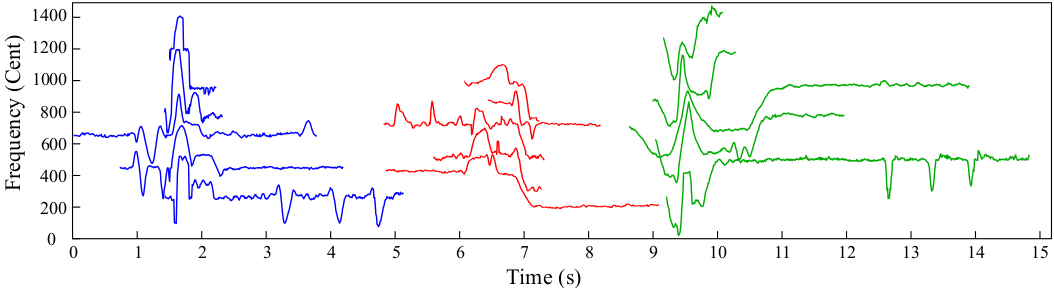
\includegraphics[scale=0.4]{carnatic_phrases.png}
  \caption{Pitch contours of occurrences of three different characteristic melodic phrases in Hindustani music. Contours are transposed in frequency, and shifted in time for a better visualization (from \cite[p.21]{gulati}).}
  \label{fig:carnatic-phrases}
\end{figure}


For all this reasons, r\=aga definition (and therefore also detection and classification) is a highly specialized task that requires a broad domain-specific knowledge, as well as a fine sense. When automating this task, a data-driven approach seems the most reasonable way of tackling it, since, except from the svaras, all the core concepts of a r\=aga can only be defined through context-depended, interconnected sets of examples.


\subsection{T\=a\d{l}a: The Rhythmic Framework}

``Tala is the rhythmic framework governing the temporal aspect of the carnatic music and it can be described as having a certain number of time units or beats (matras) and more importantly sections into which these beats are grouped and stressed''\cite{indian-corpora}.\\

The main difference between the rhythmic frameworks of western and carnatic music (apart from the fact that the latter follows an oral tradition), is that western music subdivides the temporal units from top to bottom, whereas carnatic music does the opposite. Western music follows an approach developed in the Middle Ages, in which each value could be subdivided in three (perfect division) or two (imperfect division) values of equal duration\cite[ch.XIV]{hoppin}. This system naturally evolved to allow more complex relations, but the hierarchical organization remained top down ever since then. Carnatic music builds its rhythmic abstractions by putting together rhythmic elements of shorter duration. Therefore, this section will explain those elements following that order.

\subsubsection{Layas}


Another main difference between western and carnatic music is that the former usually relates the speed to a mathematical value, by taking a specific rhythmic figure and assigning a speed to it, usually in beats per minute. And this speed is basically unrelated to the melodic or harmonic contents that the music may present.\\

In carnatic music, on the other side, ``speed is not equal to an exact mathematical value. It is generally measured as slow, medium or fast (chauka, madhyama, durita). In a generic sense, laya refers to this sense of speed, and is critical to the aesthetics of Karnatik music. The raga form is shaped on the basis of this sense and changes according to this sensed speed''\cite[p.61]{krishna}. Also, the laya of a rhythmic phenomenon ``is not experiencedby a measurable number, but by a general sense of time''\cite[p.61]{krishna}.\\

And further: ``Other tha a general sense of speed, laya also refers to the measure of the interval between every division [...]. When laya comes together with a fixed number of divisions, a composite rhythmic unit, or a tala, is created. A tala is a concrete method of dividing time [...]. Pulsation is found in many places, but it is not considered a tala unless it is created by melody''\cite[p.63]{krishna}.\\

So, after this considerations, it can be said that laya describes a general, emotional sense of rapidness provided by a rhythmic pattern, and only when the pattern becomes predictable and embodies some intentionality can be perceived as a t\=a\d{l}a.

\subsubsection{Kriyas and T\=a\d{l}a Angas}

The predictability of a rhythmic pattern is given by its periodicity: ``Every tala is cyclical in that it repeats its form in exactly the same way right through a composition''\cite[p.63]{krishna}. The layas in this context become then measurable, due to that periodicity, and are known as kriyas.\\

Kriyas are the basic building blocks of a t\=a\d{l}a, and take the form of physical manifestations ``by which both the musician and the listener can identify the tala structure''\cite[p.63]{krishna}. They can be of two types: ``those that make a sound (sashabda kriya), and those that make no sound (nishabda kriya), the first kriya in every tala is referred to as the sama -- the beginning, always the slap on the thigh''\cite[p.64]{krishna}.\\

Kriyas are combined in three structural groups, known as t\=a\d{l}a angas: ``laghu (a slap on the thigh followed by finger counts of 2,3,4,6 or 8 units), druta (a slap on the thigh followed by a flip of the palm) and anudruta (only a slap on the thigh). While druta always has two beats and anudruta one, the laghu is a variable form that can have 3,4,5,7 or 9 beats. This values are essential to all the different tala structures and the laya''\cite[p.64]{krishna}.\\

All the angas have a fixed length, except laghu, that presents ``five j\=atis (categories): chaturashra (with length 4), tisra (length 3), mishra (length 7), khanda (length 5), sankirna (length 9)''\cite[p.64]{krishna}.\\


\subsubsection{Avartanas and T\=a\d{l}as}

The t\=a\d{l}as are formed by combining few t\=a\d{l}a angas into a ``complete tala form called avartana, that is repeated cyclicaly within a specific musical representation''\cite[p.64]{krishna}. If wanting to build an analogy to western music, the role of the avartana would be similar to the measure in a baroque dance suite: the sarabande is a slow dance with has three units (with a stress in the second one) subdivided in groups of two, the gigue is a fast dance with two units (with a stress in the first one) subdivided in groups of three, and so on.\\

``In Karnatik music, there are seven talas that form the basis for the tala structures [...], known as the suladi sapta tala. Most talas in use today are variations of these seven primary talas''\cite[p.64]{krishna}. The suladi sapta talas are pictured in Table \ref{fig:taalas}.


\begin{table}
  \centering
  \resizebox{\textwidth*7/8}{!}{%
    \begin{tabular}{*3c}\toprule
      \bfseries Tala & \bfseries Structure & \bfseries Total\\\Midrule
      Dhruva  & Laghu (4) + Laghu (4) + Druta (2) + Laghu (4)    & 14 \\\midrule
      Matya   & Laghu (4) + Druta (2) + Laghu (4)                & 10  \\\midrule
      Rupaka  & Druta (2) + Laghu (4)                            & 6  \\\midrule
      Jhampa  & Laghu (7) + Anudruta (1) + Druta (2)             & 10  \\\midrule
      Triputa & Laghu (3) + Druta (2) + Druta (2)                & 7  \\\midrule
      Ata     & Laghu (5) + Laghu (5) + Druta (2) + Druta (2)    & 14 \\\midrule
      Eka     & Laghu (4)                                        & 4 \\\bottomrule
  \end{tabular}}
  \caption{The seven primary talas (from \cite[p.65]{krishna}).}
  \label{fig:taalas}
\end{table}



\subsubsection{Final Considerations}

After this considerations, it is fairly safe to say that t\=a\d{l}as are much easier to identify than r\=agas: not only there are much fewer types (as it can be seen in appendix \ref{ds-stats}), but their features are also simpler and much less context-dependent. The identification of the different angas is an easier task compared to, for instance, the gamakas. Given a basic beat of fixed duration, They comprise a fixed amount of beats (among a limited range of options) and they start with a specific gesture, the slap, which is identifiable not only visually but also audibly. When automating this task, there is an added difficulty coming from the fact that not every instrument is repeating the exact same pattern in every avartana, but this can be overcomed by exploiting two main redundancies: first, the periodicity of the avartana itself, which is kept constant thorough the whole piece, and second, the fact that all the instruments of the ensemble are following the same t\=a\d{l}a.
